%%%%%%%%%%%%%%%%%%%%%%%%%%%%%%%%%%%%%%%%%%%%%%%%%%%%%%%%%
%%             东南大学数电实验报告 LaTeX 模板
%%                SEU-Circuit-Report.cls
%% https://github.com/Teddy-van-Jerry/SEU_Digital_Report
%% ======================================================
%% 版本信息:
%% v1.0 (Nov. 07, 2021)
%% ------------------------------------------------------
%% 模板制作:
%% Teddy van Jerry, (me@teddy-van-jerry.org)
%% * GitHub: https://github.com/Teddy-van-Jerry
%% * Website: https://teddy-van-jerry.org
%% * Blog: https://blog.teddy-van-jerry.org
%% ------------------------------------------------------
%% 使用说明:
%% 1. 编译使用 XeLaTeX 和 Biber
%% 2. 报告基本信息通过修改导言区以 exp 开头的命令
%% 3. 参考文献位于 ref/ref.bib
%% 4. 报告模板依据 MIT License 开源共享
%% ------------------------------------------------------
%% Copyright 2021 (c) Teddy van Jerry
%%
%% Permission is hereby granted, free of charge, to any
%% person obtaining a copy of this software and
%% associated documentation files (the "Software"), to
%% deal in the Software without restriction, including
%% without limitation the rights to use, copy, modify,
%% merge, publish, distribute, sublicense, and/or sell
%% copies of the Software, and to permit persons to whom
%% the Software is furnished to do so, subject to the
%% following conditions:
%%
%% The above copyright notice and this permission notice
%% shall be included in all copies or substantial
%% portions of the Software.
%% 
%% THE SOFTWARE IS PROVIDED "AS IS", WITHOUT WARRANTY OF
%% ANY KIND, EXPRESS OR IMPLIED, INCLUDING BUT NOT
%% LIMITED TO THE WARRANTIES OF MERCHANTABILITY, FITNESS
%% FOR A PARTICULAR PURPOSE AND NONINFRINGEMENT. IN NO
%% EVENT SHALL THE AUTHORS OR COPYRIGHT HOLDERS BE LIABLE
%% FOR ANY CLAIM, DAMAGES OR OTHER LIABILITY, WHETHER IN
%% AN ACTION OF CONTRACT, TORT OR OTHERWISE, ARISING
%% FROM, OUT OF OR IN CONNECTION WITH THE SOFTWARE OR THE
%% USE OR OTHER DEALINGS IN THE SOFTWARE.
%%%%%%%%%%%%%%%%%%%%%%%%%%%%%%%%%%%%%%%%%%%%%%%%%%%%%%%%%%

%% 使用实验报告模板类(字体大小 11pt 约为五号字)
\documentclass[11pt]{SEU-Digital-Report}

%%%%%%%%%%%%%%%%%%%% 报告基本信息 %%%%%%%%%%%%%%%%%%%%
\expno{十一} % 实验序号
\expname{定时中断} % 实验名称
\expauthor{薛宇飞} % 姓名
\expID{04020235} % 学号
\expmates{} % 同组
\expmatesID{} % 学号(同组)
\expmajor{信息工程} % 专业
\explab{金智楼硬件实验室} % 实验室
\expdate{\today} % 实验日期
\expreportdate{\today} % 实验日期
\expgrade{} % 成绩评定
\exptutor{裴文江} % 评阅教师
%%%%%%%%%%%%%%%%%%%%%%%%%%%%%%%%%%%%%%%%%%%%%%%%%%%%
% \usepackage{xeCJK}
\usepackage{threeparttable} %table添加注释
\usepackage{colortbl}
\newcommand{\grayrow}{\rowcolor[rgb]{ .906, .902, .902}}
\usepackage{xcolor}  % tikz画图
\usepackage{tikz}  
\usetikzlibrary{arrows,shapes,chains} 
\usepackage{pgfplots}
\pgfplotsset{compat=1.11}

%% 报告正文
\begin{document}

% 打印封面页
\exptitlepage

\tableofcontents
\newpage

\section{实验目的与内容}       
\begin{enumerate}
    \item 结合实验教材\cite{book,guide},熟悉\texttt{Intel 8086CPU}的中断处理功能以及IBM-PC的中断结构.
    \item 了解\texttt{8253}定时器的使用.
    \item 掌握定时中断的编程,观察中断的执行情况. 
\end{enumerate}

\section{实验任务}
\subsection{基本功能}
定时/计数器\texttt{8253}每隔\texttt{55ms}发一次定时中断请求信号(其中断类型号为\texttt{1CH}), CPU响应中断后转去执行\texttt{TIMERINTS}中断服务程序。

本次实验任务为改写定时中断(中断类型号为\texttt{1CH})的中断服务程序,要求在定时中断服务程序中累计中断次数,每计到50次定时中断就在显示器上显示字符串\texttt{“SUN”}。

主程序:从屏幕左上角到右下角循环显示“太阳”图形,并判断字符串“SUN”的显示次数是否到十次,到十次就结束程序返回DOS。



\subsection{附加任务}
\begin{enumerate}
    \item 定时1秒左右显示一次\texttt{“SUN”},并在显示\texttt{”SUN”}的前面加上显示次数;
    \item 显示10次\texttt{”SUN”}后,不等25行太阳图标显示完,立即返回\texttt{DOS};
    \item 在本次实验中加入实验十的键盘中断,如果有按键,就显示\texttt{“KEY”}(前面加上显示次数);每定时1秒左右就显示一次\texttt{“SUN”}(前面加上显示次数)。按键或显示\texttt{“SUN”}只要有一个到10次了,就结束程序返回\texttt{DOS}。
    \item 修改显示字符的属性,如,红底白字,蓝底黄字…… 
\end{enumerate}

\section{实验原理}
在主程序中应先保存原中断类型号1CH的中断服务程序入口地址,然后把自行编写的\texttt{TIMERINTS}定时中断服务程序入口地址的段内偏移地址和段地址存入以\texttt{1CH*4}为起始地址的四个连续单元内。

主程序中安排开中断指令,\texttt{CPU}响应中断后自动转入\texttt{TIMERINTS}定时中断服务程序去执行。    

主程序和定时中断服务程序流程图如图\ref{fig:process}所示。

\begin{figure}[htbp]
    \centering
    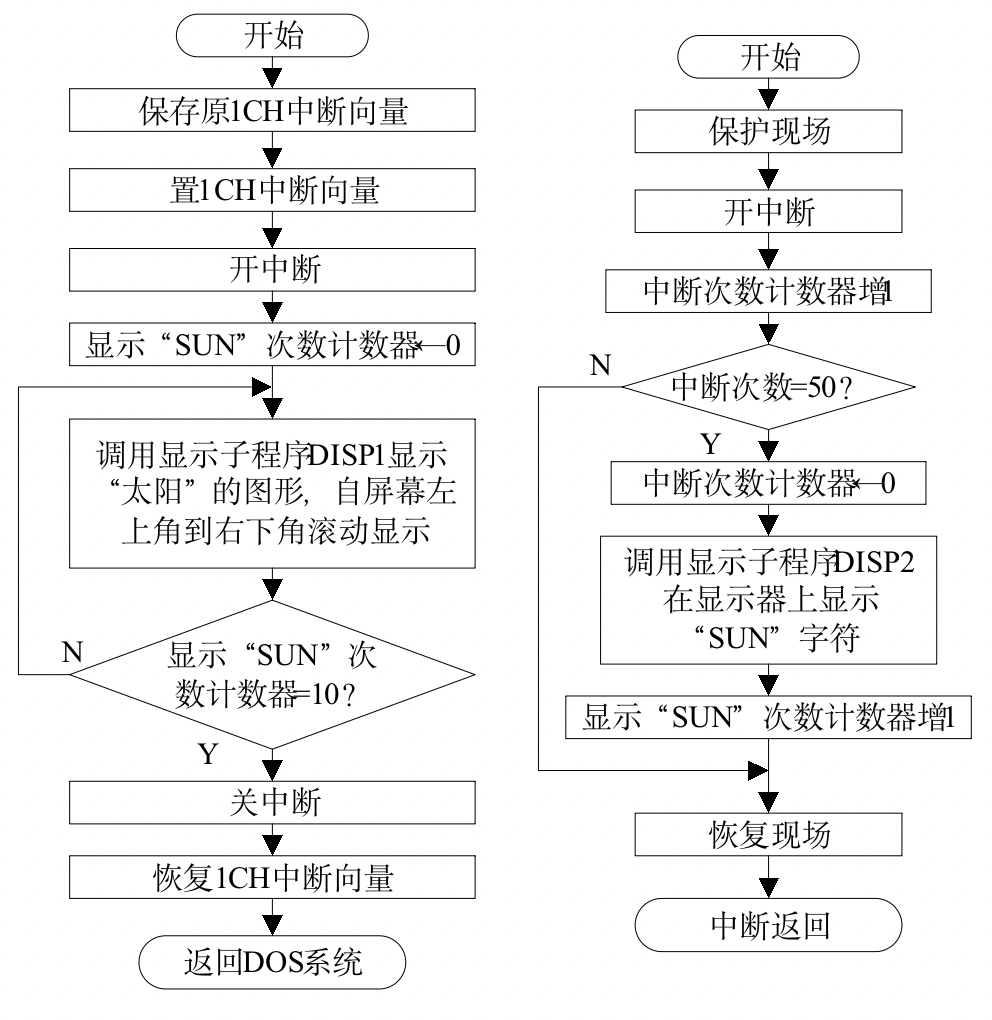
\includegraphics[width=0.7\textwidth]{fig/process.png}
    \caption{流程图}
    \label{fig:process}
\end{figure}

自屏幕左上角向右下角移动并显示“太阳”图形的显示子程序如下: 
\begin{lstlisting}[language={[x86masm]Assembler},title=code]
    DISP1  PROC  FAR
        PUSH   AX
        PUSH   BX
        PUSH   CX
        PUSH   DX
        MOV    AH,15    ;读当前显示状态,
        INT    10H
        MOV    AH,0     ;设置显示方式
        INT    10H
        MOV    CX,1     ;显示的字符个数为1
        MOV    DX,0     ;行号为0,列号为0
    REPT: 
        MOV    AH,2      ;设置光标位置
        INT    10H
        MOV    AL,0FH    ;读出太阳图形
        MOV    AH,10     ;写字符
        INT    10H
        CALL   DELAY
        SUB    AL,AL
        MOV    AH,10      ;清除原图形
        INT    10H
        INC    DH
        ADD    DL,2
        CMP    DH,25
        JB    REPT
        POP    DX
        POP    CX
        POP    BX
        POP    AX    
        RET
    DISP1   ENDP
\end{lstlisting}

在定时中断服务程序中显示字符串“SUN”的子程序DISP2程序如下:
\begin{lstlisting}[language={[x86masm]Assembler},title=code]
    DISP2  PROC   FAR
        PUSH   CX    
        PUSH   BX
        PUSH   AX
        MOV    CX,10
    NEXTC: 
        LODSB
        MOV   AH,0EH
        MOV   BX,01
        INT    10H
        CALL   DELAY
        LOOP   NEXTC
        POP    AX
        POP    BX
        POP    CX
        RET
    DISP2    ENDP
\end{lstlisting}

延时子程序(延时大约1秒左右)如下:
\begin{lstlisting}[language={[x86masm]Assembler},title=code]
    DELAY  PROC  FAR
        PUSH   CX
        PUSH   DX
        MOV    DX,20
    DL500:
        MOV    CX,0FFFFH
    DL10ms:
        LOOP  DL10ms
        DEC    DX
        JNZ    DL500
        POP    DX
        POP    CX
        RET
    DELAY   ENDP
\end{lstlisting}

\section{实验代码}
\begin{lstlisting}[language={[x86masm]Assembler},title=code]
    DATA SEGMENT
        TIMES_COUNTS DB ?
        SUN_COUNTS DB ?
        SUN_PRINT DB "    SUN"
        KEY_COUNTS DB ?
        OK_PRINT DB "    OK!"           ;字符串中的空格为按键次数预留(两个数字+两个空格+OK!)
    DATA ENDS

    STACK SEGMENT                                   ;为保护现场操作建立栈段空间
        DW 10 DUP(?)
    STACK ENDS

    CODE SEGMENT
    ASSUME CS:CODE,DS:DATA,ES:DATA,SS:STACK
    START:
        MOV AX,STACK
        MOV SS,AX
        MOV AX,DATA
        MOV DS,AX
        MOV AX,0000H                              ;设置中断向量操作
        MOV ES,AX
        MOV SI,1CH*4
        PUSH ES:[SI+2]                              ;保存原1CH中断向量
        PUSH ES:[SI]
        MOV WORD PTR ES:[SI+2],SEG TIMERINTS     ;设置新1CH中断向量
        MOV WORD PTR ES:[SI],OFFSET TIMERINTS

        MOV AL,09H                              ;用中断类型21H的35H功能取中断向量保存
        MOV AH,35H
        INT 21H
        PUSH ES
        PUSH BX
        MOV DX,OFFSET KEYINTS                   ;用中断类型21H的25H功能设置中断向量
        MOV AX,SEG KEYINTS
        MOV DS,AX
        MOV AL,09H
        MOV AH,25H
        INT 21H
        MOV AX,DATA                             ;恢复数据段地址
        MOV DS,AX

        STI                                         ;开中断
        MOV TIMES_COUNTS,00H                    ;定时中断次数置零
        MOV SUN_COUNTS,00H                      ;输出“SUN”次数置零
        MOV KEY_COUNTS,00H                      ;按键次数置零
    SUN:
        CALL DISPl                                   ;输出太阳
        MOV AL,SUN_COUNTS   
        SUB AL,10                          ;sun次数-10,放入al 
        MOV AH,KEY_COUNTS
        SUB AH,10                           ;key次数-10,放入ah

        AND AL,AH                               ;只要有一个达到10,结果为0
        CMP AL,0
        ;CMP SUN_COUNTS,10                          ;比较输出“SUN”次数
        ;CMP KEY_COUNTS,10                           ;比较按键次数
        JNE SUN                                        ;不等于,继续输出太阳

        CLI                                          ;关中断
        MOV SI,1CH*4          
        POP ES:[SI]                                   ;恢复原1CH中断向量
        POP ES:[SI+2]

        POP DX                                  ;用中断类型21H的25H功能恢复中断向量,回顾line32 33
        POP DS
        MOV AL,09H
        MOV AH,25H
        INT 21H      

        MOV AH,4CH                                 ;返回DOS
        INT 21H

    TIMERINTS PROC NEAR
        PUSH AX                                     ;保护现场
        PUSH BX
        PUSH DX
        PUSH SI
        STI                                           ;开中断
        INC TIMES_COUNTS                           ;定时中断次数+1
        CMP TIMES_COUNTS,50                       ;定时中断次数未到50不输出“SUN”;定时1s可以计算得1s/55ms=18
        JB PASS                                     ;低于
        MOV TIMES_COUNTS,00H                      ;定时中断次数清零,重新累加
        INC SUN_COUNTS                             ;输出“SUN”次数+1

        MOV AL, SUN_COUNTS
        ADD AL, 30H                                 ;将按键次数转换为ASCII码,以便输出
        CMP AL, 3AH
        JNE PRINT

        MOV SUN_PRINT, 31H                           ;按键次数为10的ASCII码,10是两位数,单独设置一下
        MOV SUN_PRINT+1, 30H
        JMP CHGSI

        LEA SI,SUN_PRINT                            ;取“SUN”偏移地址,准备输出
        CALL DISP2
    PRINT:  
        MOV SUN_PRINT, AL
    CHGSI:  
        LEA BP,SUN_PRINT                             ;为DISP2中进行INT 10H中断作预处理
        MOV AX,SEG SUN_PRINT                        
        MOV ES,AX
        CALL DISP2
    PASS:
        POP SI                                       ;恢复现场
        POP DX
        POP BX
        POP AX      
        IRET                                         ;中断返回
    TIMERINTS ENDP

    DISPl PROC NEAR
        PUSH  AX                                    ;保护现场
        PUSH  BX
        PUSH  CX
        PUSH  DX
        MOV AH,15                                   ;读当前显示状态,放入AL
        INT 10H
        MOV AH,0                                    ;设置显示方式: AL=显示方式号; 起到清屏的作用
        INT 10H
        MOV CX,1                                    ;设置显示字符的个数
        MOV DX,0                                    ;设置行列为0
    REAPT:
        MOV AH,2                                   ;设置光标位
        INT 10H


        MOV AL,SUN_COUNTS   
        SUB AL,10                          ;sun次数-10,放入al 
        MOV AH,KEY_COUNTS
        SUB AH,10                           ;key次数-10,放入ah

        AND AL,AH                               ;只要有一个达到10,结果为0
        CMP AL,0
        JE PASS1                                  ;次数达到要求则不再输出太阳


        MOV AL,0FH                                 ;读出太阳图形
        MOV AH,10                                  ;设置功能号,写字符
        INT 10H
        CALL DELAY                                 ;调用延时子程序
        SUB AL,AL
        MOV AH,10                                  ;清除原图形
        INT 10H
        INC DH
        ADD DL,2                                    
        CMP DH,25                                  ;未输出完1页以前,持续输出
        JNE REAPT
    PASS1:
        POP DX                                    ;恢复现场
        POP CX
        POP BX
        POP AX
        RET
    DISPl ENDP

    DISP2 PROC NEAR
        PUSH CX                                    ;保护现场
        PUSH BX
        PUSH AX
        PUSH DX
        ;MOV BH, 00H                                
        MOV AH, 03H                                ;获取光标位置: BH=page number(default=0), DH=row number, DL=column number
        INT 10H
        MOV CX,7                                   ;显示字符串长度,包含了按键次数和空格,故需要七个(与数据段对应)
        MOV AH,13H                                 ;用AH=13H的INT 10H中断改变字体颜色
        MOV BL,4FH                                 ;certain color
        MOV BH,00H                                 ;Page number
        MOV AL,01H
        INT 10H                                   
        ;CALL DELAY
        POP DX
        POP AX                                    ;恢复现场
        POP BX
        POP CX
        RET
    DISP2 ENDP

    DELAY PROC NEAR                               ;延时1秒子程序
        PUSH CX
        PUSH AX
        MOV AL,23
    GOONN:MOV CX,0FFFFH	;实现延时1秒
    GOON:DEC CX 
        JNZ GOON
        DEC AL
        CMP AL,00
        JNE GOONN
        MOV CX,0004H
    GOONE:DEC CX
        JNZ GOONE
        POP AX
        POP CX
        RET
    DELAY ENDP

    ;键盘中断子程序
    KEYINTS PROC NEAR
        PUSH AX                                     ;保护现场
        PUSH BX
        PUSH DX
        PUSH SI

        STI                                         ;开中断

        IN AL,60H                                   ;读取键盘扫描码(ASCII存放在AL)
        MOV AH,AL                                   ;保护键盘扫描码               
        IN AL,61H                                   ;PB口的当前键盘ASCII值
        OR AL,80H                                   ;PB7置1,产生中断请求信号(脉冲信号)
        OUT 61H,AL
        AND AL,7FH                                  ;PB7置0,为下一次读取扫描码做准备
        OUT 61H,AL

        TEST AH,80H                                 ;根据扫描码判断按键为按下还是松开
        JNE PASS_KEY                                   ;不等于,为松开状态,则不计按键数,不输出OK,跳到PASS


        MOV AL,SUN_COUNTS   
        SUB AL,10                          ;sun次数-10,放入al 
        MOV AH,KEY_COUNTS
        SUB AH,10                           ;key次数-10,放入ah

        AND AL,AH                               ;只要有一个达到10,结果为0
        CMP AL,0

        ;CMP KEY_COUNTS,10                           ;保证按键达到十次后结束程序
        JE PASS_KEY                      
        INC KEY_COUNTS                              ;按键数+1               ;
        MOV AL, KEY_COUNTS
        ADD AL, 30H                                 ;将按键次数转换为ASCII码,以便输出
        CMP AL, 3AH
        JNE PRINT_OK

        MOV OK_PRINT, 31H                           ;按键次数为10的ASCII码,10是两位数,单独设置一下
        MOV OK_PRINT+1, 30H
        JMP CHGSI_OK
    PRINT_OK:  
        MOV OK_PRINT, AL
    CHGSI_OK:  
        LEA BP,OK_PRINT                             ;为DISP2中进行INT 10H中断作预处理
        MOV AX,SEG OK_PRINT                        
        MOV ES,AX
        CALL DISP_OK
    PASS_KEY:
        MOV AL,20H                                 ;发出中断结束命令
        OUT 20H,AL
        POP SI                                     ;恢复现场
        POP DX
        POP BX
        POP AX
        ;STI                                        ;开中断
        IRET                                       ;中断返回
    KEYINTS ENDP

    DISP_OK PROC NEAR
        PUSH CX                                    ;保护现场
        PUSH BX
        PUSH AX
        PUSH DX

        ;MOV BH, 00H                                
        MOV AH, 03H                                ;获取光标位置: BH=page number(default=0), DH=row number, DL=column number
        INT 10H
        MOV CX,7                                   ;显示字符串长度,包含了按键次数和空格,故需要七个(与数据段对应)
        MOV AH,13H                                 ;用AH=13H的INT 10H中断改变字体颜色
        MOV BL,2CH                                 ;certain color
        MOV BH,00H                                 ;Page number
        MOV AL,01H
        INT 10H                                   
        ;CALL DELAY
        POP DX
        POP AX                                    ;恢复现场
        POP BX
        POP CX
        RET
    DISP_OK ENDP

    CODE ENDS
    END START
\end{lstlisting}

\section{实验结果}
实验中,完成附加任务后,因定时中断、键盘中断返回\texttt{DOS}的效果图如图\ref{fig:rst1}和图\ref{fig:rst2}.
\begin{figure}[htbp]
    \centering
    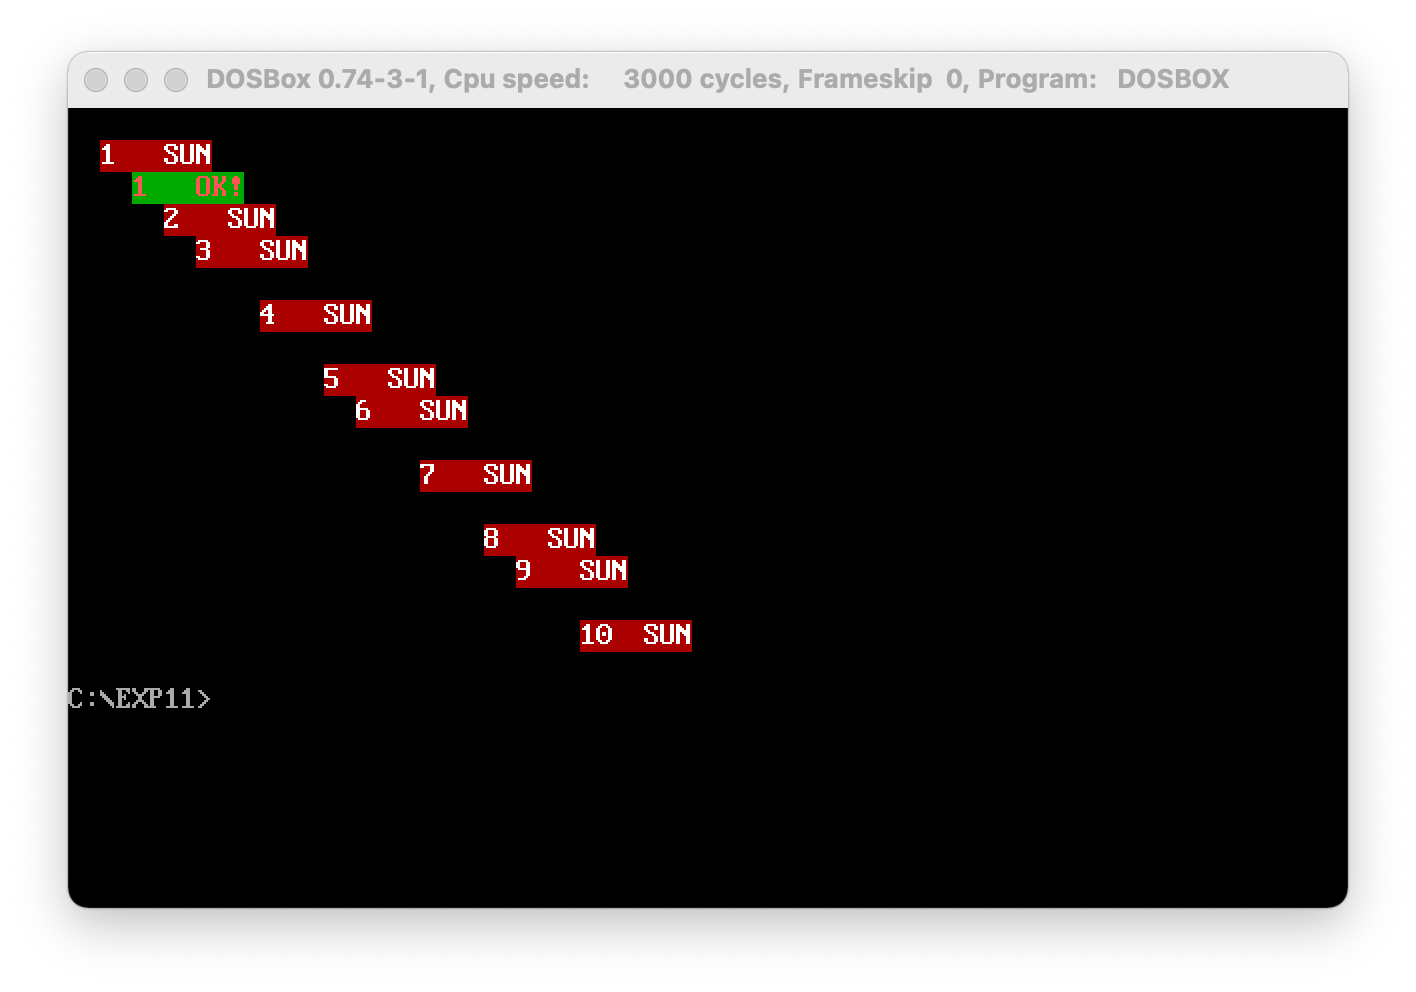
\includegraphics[width=0.7\textwidth]{fig/rst1.png}
    \caption{result-1}
    \label{fig:rst1}
\end{figure}

\begin{figure}[htbp]
    \centering
    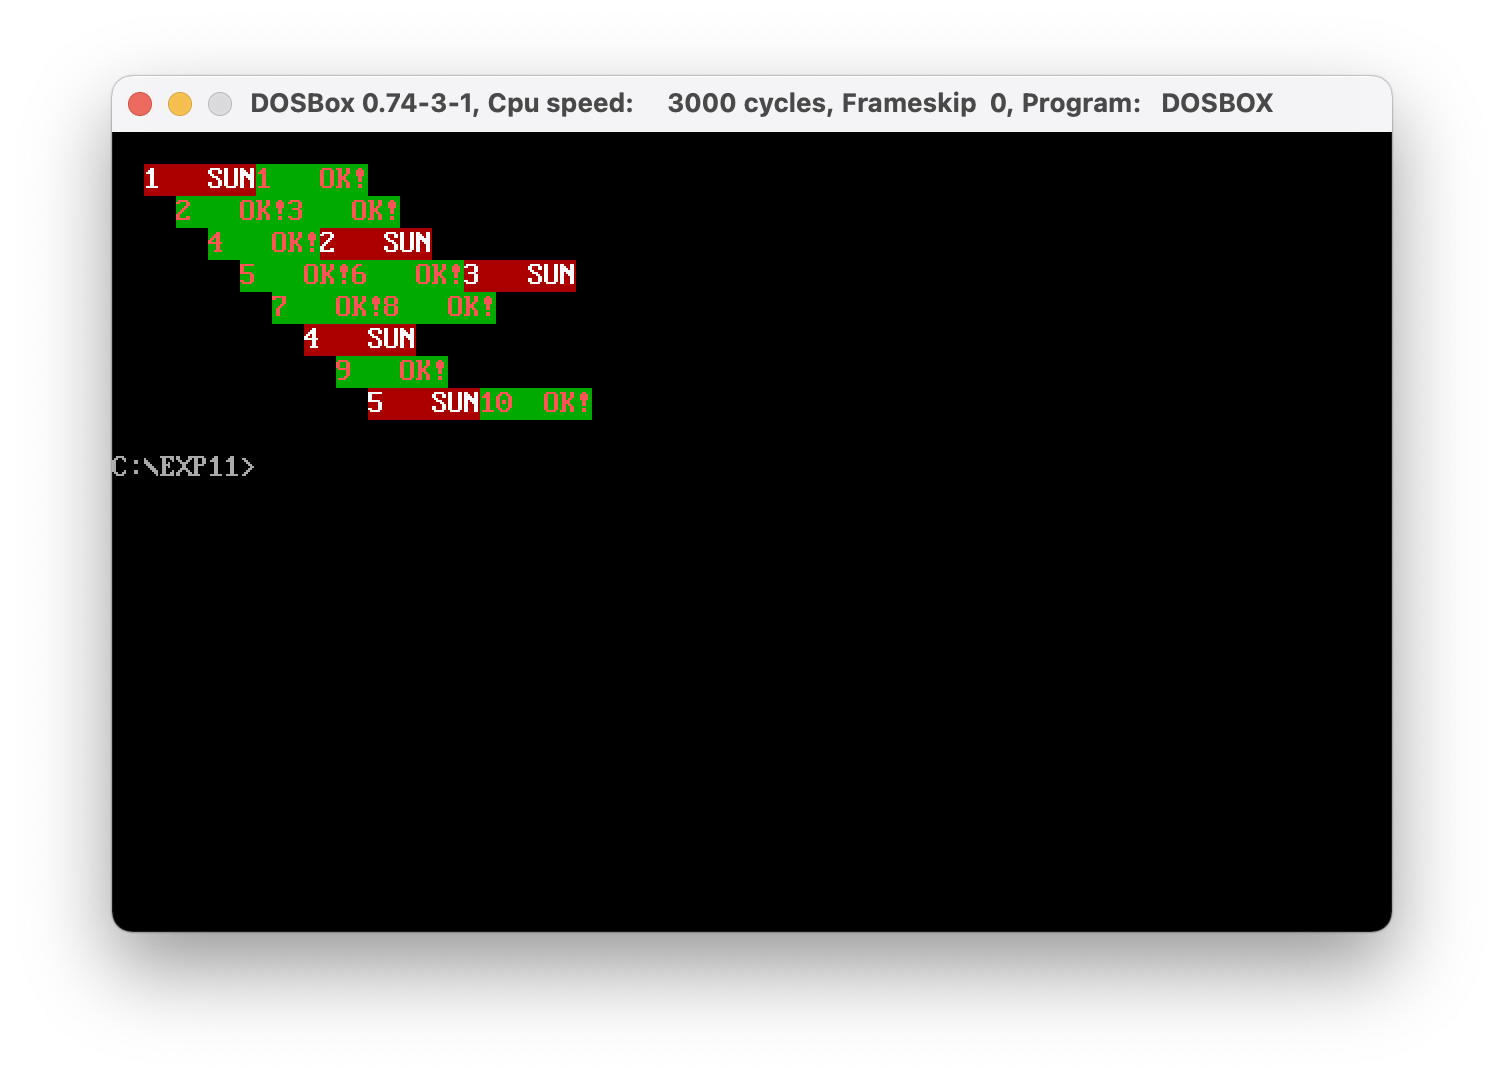
\includegraphics[width=0.7\textwidth]{fig/rst2.png}
    \caption{result-2}
    \label{fig:rst2}
\end{figure}

\section{附加任务说明}
\subsection{附加任务1}
由于\texttt{1s/55ms=18},故应该累计18次显示一次“\texttt{SUN}”,将\texttt{TIMERINTS}子程序中的\texttt{CMP}语句的源操作数改为18即可,即
\begin{lstlisting}[language={[x86masm]Assembler},title=code]
    TIMERINTS PROC NEAR
    PUSH AX                                     ;保护现场
    PUSH BX
    PUSH DX
    PUSH SI
    STI                                           ;开中断
    INC TIMES_COUNTS                           ;定时中断次数+1
    CMP TIMES_COUNTS, 18                       ;定时中断次数未到18不输出“SUN”
    JB PASS
    MOV TIMES_COUNTS,00H                      ;定时中断次数清零,重新累加
    LEA SI,SUN_PRINT                            ;取“SUN”偏移地址,准备输出
    CALL DISP2
    INC SUN_COUNTS                             ;输出“SUN”次数+1
    PASS:
    POP SI                                       ;恢复现场
    POP DX
    POP BX
    POP AX      
    IRET                                         ;中断返回
    TIMERINTS ENDP
\end{lstlisting}
\subsection{附加任务2-3}
由于后续需要假如键盘中断,所以我们综合来看附加任务2-3,定时中断或者键盘中断任意一个达到10次需要返回\texttt{DOS},这要求需要对两个次数综合判断,即
\begin{lstlisting}[language={[x86masm]Assembler},title=code]
    CALL DISPl                                   ;输出太阳
    MOV AL,SUN_COUNTS   
    SUB AL,10                          ;sun次数-10,放入al 
    MOV AH,KEY_COUNTS
    SUB AH,10                           ;key次数-10,放入ah

    AND AL,AH                               ;只要有一个达到10,结果为0
    CMP AL,0
    ;CMP SUN_COUNTS,10                          ;比较输出“SUN”次数
    ;CMP KEY_COUNTS,10                           ;比较按键次数
    JNE SUN     
\end{lstlisting}
该结果需要在打印\texttt{SUN}和\texttt{OK!}都需要判断,所以需要将此程序段插入所有判断次数的位置,通过运行可以得到正确的结果。

\subsection{附加任务4}
修改字体颜色需要调用\texttt{INT 10H}的\texttt{13H}功能:
\begin{note}{\texttt{INT 10H}的\texttt{13H}功能}{}
    \texttt{BH}=页码

    \texttt{BL}=属性(若\texttt{AL}=\texttt{00H}或\texttt{01H})

    \texttt{CX}=显示字符串长度

    (\texttt{DH}、\texttt{DL})=坐标(行、列)

    \texttt{ES:BP}=显示字符串的地址 AL=显示输出方式

    0: 字符串中只含显示字符,其显示属性在BL中.显示后,光标位置不变

    1: 字符串中只含显示字符,其显示属性在BL中.显示后,光标位置改变

    2: 字符串中含显示字符和显示属性.显示后,光标位置不变

    3: 字符串中含显示字符和显示属性.显示后,光标位置改变
\end{note}
由此得到的代码为:
\begin{lstlisting}[language={[x86masm]Assembler},title=code]
    DISP_OK PROC NEAR
        PUSH CX                                    ;保护现场
        PUSH BX
        PUSH AX
        PUSH DX

        ;MOV BH, 00H                                
        MOV AH, 03H                                ;获取光标位置: BH=page number(default=0), DH=row number, DL=column number
        INT 10H
        MOV CX,7                                   ;显示字符串长度,包含了按键次数和空格,故需要七个(与数据段对应)
        MOV AH,13H                                 ;用AH=13H的INT 10H中断改变字体颜色
        MOV BL,2CH                                 ;certain color
        MOV BH,00H                                 ;Page number
        MOV AL,01H
        INT 10H                                   
        ;CALL DELAY
        POP DX
        POP AX                                    ;恢复现场
        POP BX
        POP CX
        RET
    DISP_OK ENDP
\end{lstlisting}
以上是打印\texttt{OK!}的程序,打印\texttt{SUN}只需要将所需字符串修改即可!
\section{思考题}
如果要求定时1秒左右显示一次“SUN”,那么,定时中断应该累计多少次显示一次“SUN”,程序应该如何修改?

由于\texttt{1s/55ms=18},故应该累计18次显示一次“\texttt{SUN}”,将\texttt{TIMERINTS}子程序中的\texttt{CMP}语句的源操作数改为18即可,具体见附加任务1。

\section{实验思考}
\begin{enumerate}
    \item [$\bullet$] 实验涉及到两个中断:定时中断和键盘中断,在编程过程中需要综合考虑判断;
    \item [$\bullet$] 刚开始运行的时候,虽然键盘按下10次可以满足退出程序返回\texttt{DOS},但是无法打印,经过思考发现是判断语句出现错误,导致按键小于10次时候没有输出直接\texttt{PASS},经过更正得到了正确的结果;
    \item [$\bullet$]在实验过程中,遇到了一种情况:在键盘按下第11次时候仍然有输出,思考原因是判断条件不完善,但是\texttt{DELAY}时长也会影响程序运行。
\end{enumerate}


% 打印参考文献
\addcontentsline{toc}{section}{参考文献}
\printbibliography

\end{document}
